In this section we compare results of the old analysis used for EPS
2011 conference~\cite{HWW2011} and the current analysis with all the
improvements including refined background estimations. The dataset is
the one used for EPS 2011 and it corresponds to $1.1\pm0.1\ifb$. 
We also show the results for the dataset corresponding to the full data
sample except the EPS one, so-called Post-EPS sample.

The expected and observed upper limits at 95\% C.L. for the cut-based and
multivariate analyses using the EPS sample are shown in 
Tables~\ref{tab:cutbase_uls_eps} and~\ref{tab:mvabase_uls_eps}, respectively. 
The corresponding exclusion limits are shown in Figure~\ref{fig:uls_eps}.

%%%%%%%%%%%%%%%%%%%%%%%%%%%%%%
\begin{table}[hbp!]
\begin{center}
\begin{tabular}{c c c c c}
\hline
\vspace{-3mm} && \\
 Higgs Mass   & Observed & Median expected & Expected range for 68\% & Expected range for 95\%   \\
    & (new/old) & (new/old) & (new/old) & (new/old)   \\
\vspace{-3mm} && \\
\hline
115 & 6.4 / 4.7 & 5.3 / 4.6 & [3.8, 7.3] / [3.3, 6.3] & [2.8, 9.8] / [2.4, 8.5] \\
120 & 4.8 / 3.8 & 3.0 / 2.9 & [2.2, 4.2] / [2.1, 4.0] & [1.6, 5.7] / [1.5, 5.3] \\
130 & 2.6 / 2.2 & 1.4 / 1.4 & [1.0, 1.9] / [1.0, 2.0] & [0.7, 2.6] / [0.8, 2.7] \\
140 & 1.4 / 1.2 & 0.9 / 0.9 & [0.6, 1.2] / [0.6, 1.2] & [0.5, 1.6] / [0.5, 1.6] \\
150 & 0.9 / 0.9 & 0.7 / 0.7 & [0.5, 0.9] / [0.5, 0.9] & [0.4, 1.2] / [0.4, 1.2] \\
160 & 0.6 / 0.5 & 0.4 / 0.4 & [0.3, 0.5] / [0.3, 0.5] & [0.2, 0.7] / [0.2, 0.7] \\
170 & 0.6 / 0.6 & 0.4 / 0.4 & [0.3, 0.6] / [0.3, 0.6] & [0.2, 0.8] / [0.2, 0.8] \\
180 & 0.6 / 0.5 & 0.5 / 0.5 & [0.4, 0.8] / [0.4, 0.7] & [0.3, 1.0] / [0.3, 1.0] \\
190 & 1.2 / 0.9 & 0.8 / 0.8 & [0.6, 1.1] / [0.6, 1.1] & [0.4, 1.5] / [0.4, 1.5] \\
200 & 1.7 / 1.3 & 1.0 / 1.1 & [0.7, 1.3] / [0.8, 1.6] & [0.5, 1.8] / [0.6, 2.1] \\
250 & 2.1 / 1.8 & 1.9 / 2.1 & [1.4, 2.7] / [1.5, 2.9] & [1.0, 3.6] / [1.1, 3.8] \\
300 & 2.6 / 2.3 & 2.3 / 2.3 & [1.7, 3.2] / [1.7, 3.2] & [1.2, 4.3] / [1.2, 4.3] \\
350 & 2.3 / 2.4 & 2.1 / 2.2 & [1.5, 3.0] / [1.6, 3.1] & [1.1, 4.0] / [1.2, 4.1] \\
400 & 2.5 / 2.4 & 2.4 / 2.5 & [1.7, 3.4] / [1.8, 3.5] & [1.3, 4.5] / [1.4, 4.7] \\
450 & 2.9 / 2.5 & 3.2 / 3.3 & [2.3, 4.5] / [2.4, 4.6] & [1.7, 6.0] / [1.8, 6.2] \\
500 & 4.3 / 3.4 & 4.7 / 4.5 & [3.4, 6.5] / [3.2, 6.2] & [2.5, 8.7] / [2.4, 8.3] \\
550 & 5.1 / 4.0 & 6.4 / 6.1 & [4.6, 8.9] / [4.4, 8.5] & [3.4, 11.9] / [3.3, 11.4] \\
600 & 7.0 / 5.4 & 9.2 / 8.7 & [6.6, 12.8] / [6.2, 12.1] & [4.9, 17.1] / [4.6, 16.2] \\

\hline
\end{tabular}
\caption{Expected and observed upper limits for SM Higgs using the
  {\bf cut-based} analysis using EPS dataset.}
\label{tab:cutbase_uls_eps}
\end{center}
\end{table}
%%%%%%%%%%%%%%%%%%%%%%%%%%%%%%

%%%%%%%%%%%%%%%%%%%%%%%%%%%%%%
\begin{table}[hbp!]
\begin{center}
\begin{tabular}{c c c c c}
\hline
\vspace{-3mm} && \\
 Higgs Mass   & Observed & Median expected & Expected range for 68\% & Expected range for 95\%   \\
  & (new/old) & (new/old) & (new/old) & (new/old)   \\
\vspace{-3mm} && \\
\hline
115 & 8.6 / 7.1 & 4.5 / 3.1 & [3.2, 6.2] / [2.2, 4.3]& [2.4, 8.4] / [1.7, 5.8] \\
120 & 4.4 / 3.5 & 2.7 / 2.0 & [2.0, 3.8] / [1.4, 2.7]& [1.5, 5.1] / [1.0, 3.6] \\
130 & 2.1 / 1.8 & 1.3 / 1.0 & [0.9, 1.8] / [0.7, 1.4]& [0.7, 2.4] / [0.5, 1.9] \\
140 & 1.4 / 1.3 & 0.8 / 0.6 & [0.6, 1.1] / [0.5, 0.9]& [0.4, 1.5] / [0.3, 1.2] \\
150 & 1.1 / 1.0 & 0.5 / 0.5 & [0.4, 0.7] / [0.3, 0.6]& [0.3, 1.0] / [0.2, 0.9] \\
160 & 0.6 / 0.6 & 0.3 / 0.3 & [0.2, 0.4] / [0.2, 0.4]& [0.2, 0.6] / [0.2, 0.5] \\
170 & 0.6 / 0.5 & 0.3 / 0.3 & [0.2, 0.5] / [0.2, 0.5]& [0.2, 0.6] / [0.2, 0.6] \\
180 & 0.8 / 0.6 & 0.5 / 0.4 & [0.3, 0.7] / [0.3, 0.6]& [0.3, 0.9] / [0.2, 0.8] \\
190 & 1.1 / 0.8 & 0.7 / 0.7 & [0.5, 1.0] / [0.5, 0.9]& [0.4, 1.3] / [0.4, 1.2] \\
200 & 1.8 / 1.3 & 0.8 / 0.9 & [0.6, 1.1] / [0.7, 1.3]& [0.4, 1.5] / [0.5, 1.7] \\
250 & 1.8 / 1.4 & 1.6 / 1.5 & [1.2, 2.2] / [1.1, 2.1]& [0.9, 3.0] / [0.8, 2.8] \\
300 & 1.5 / 1.5 & 1.9 / 1.7 & [1.3, 2.6] / [1.2, 2.3]& [1.0, 3.5] / [0.9, 3.1] \\
350 & 1.6 / 2.1 & 1.7 / 1.6 & [1.2, 2.4] / [1.2, 2.2]& [0.9, 3.2] / [0.9, 3.0] \\
400 & 2.0 / 1.6 & 1.9 / 1.7 & [1.3, 2.6] / [1.3, 2.4]& [1.0, 3.5] / [0.9, 3.2] \\
450 & 2.7 / 2.2 & 2.6 / 2.5 & [1.9, 3.6] / [1.8, 3.4]& [1.4, 4.9] / [1.3, 4.6] \\
500 & 3.0 / 2.3 & 3.8 / 3.4 & [2.7, 5.3] / [2.4, 4.7]& [2.0, 7.1] / [1.8, 6.3] \\
550 & 4.2 / 3.6 & 5.2 / 4.8 & [3.7, 7.2] / [3.4, 6.6]& [2.8, 9.7] / [2.6, 8.9] \\
600 & 5.9 / 4.9 & 7.6 / 6.9 & [5.5, 10.6] / [4.9, 9.5]& [4.1, 14.2] / [3.7, 12.8]\\

>>>>>>> 1.2
\hline
\end{tabular}
\caption{Expected and observed upper limits for SM Higgs using the
  {\bf shape-based} analysis using EPS dataset.}
\label{tab:mvabase_uls_eps}
\end{center}
\end{table}

\begin{figure}[!hbtp]
\centering
\subfigure[SM Higgs (cut-based)]{
\centering
\label{subfig:sm_cut}
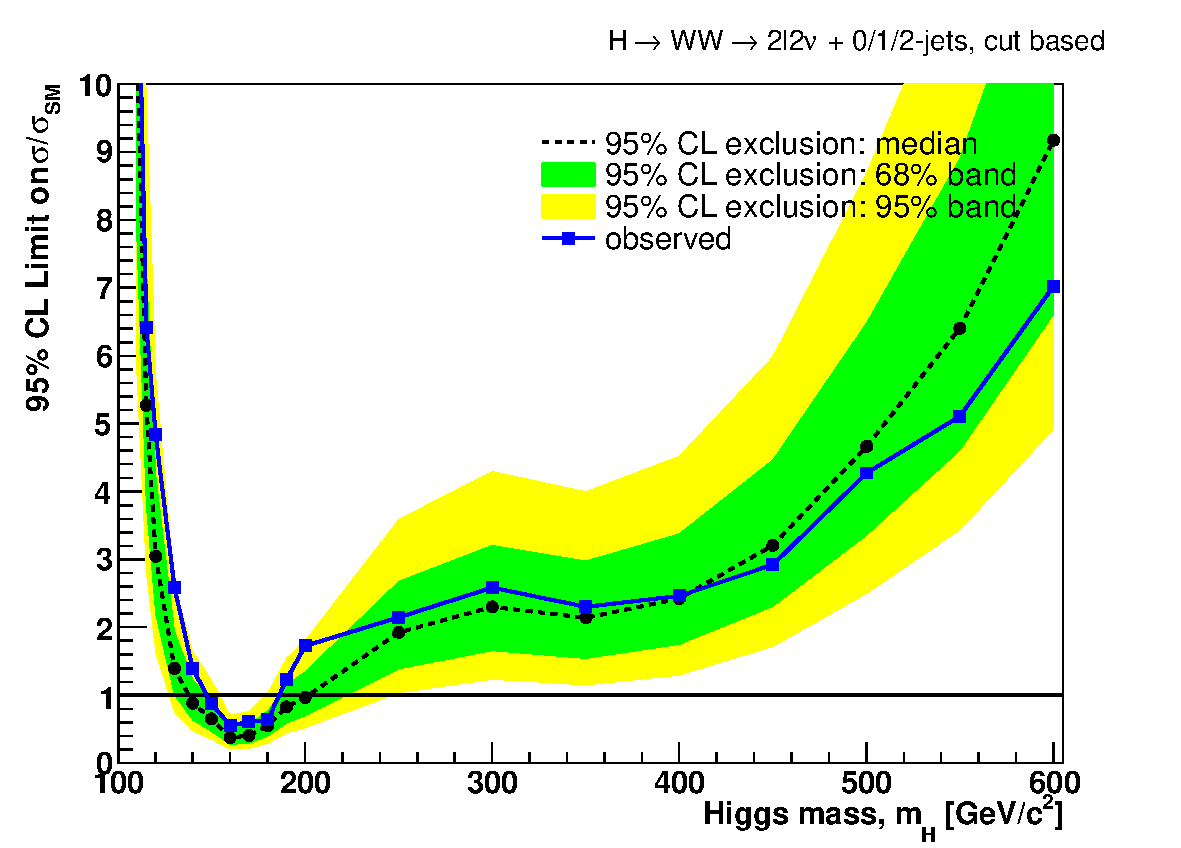
\includegraphics[width=.45\textwidth]{figures/limits_nj_cut-CLs-asymptotic_EPS.pdf}}
\subfigure[SM Higgs (shape-based)]{
\centering
\label{subfig:sm_cut_zoom}
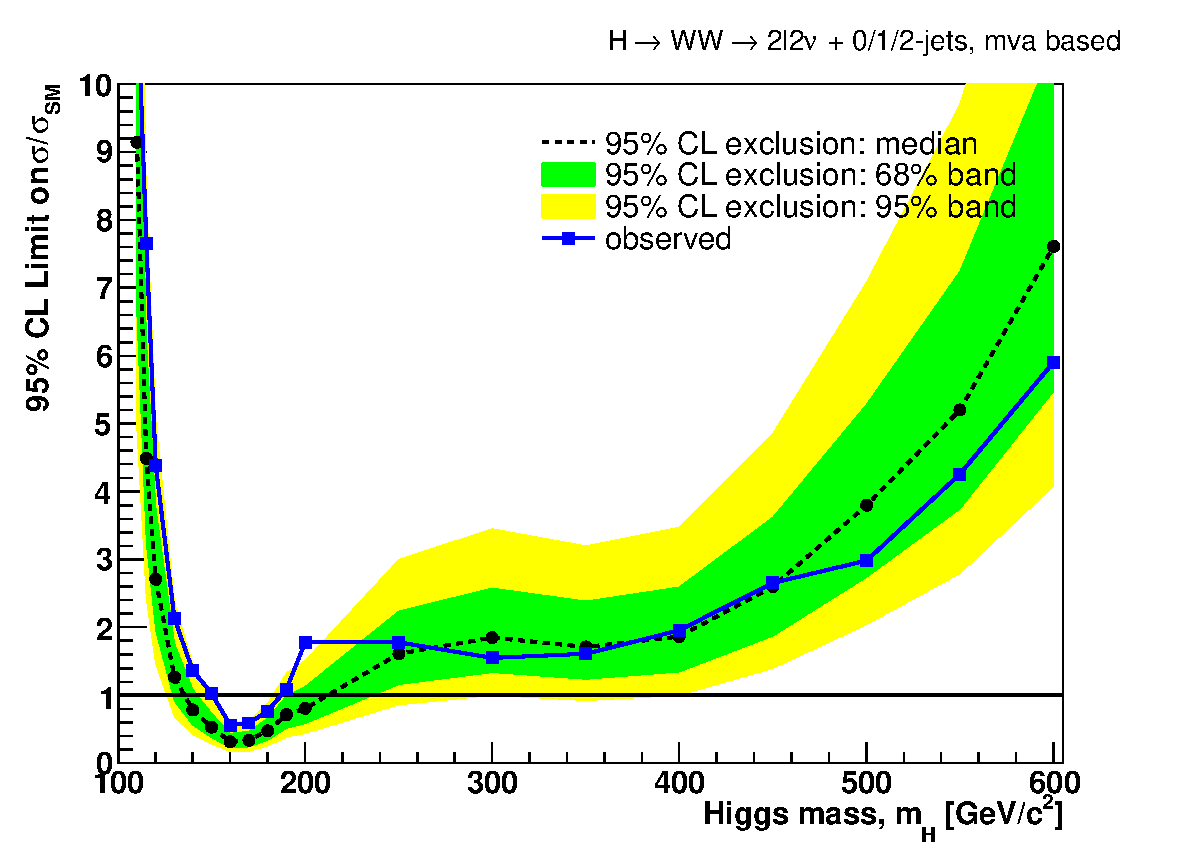
\includegraphics[width=.45\textwidth]{figures/limits_nj_shape-CLs-asymptotic_EPS.pdf}}

\caption{Expected and observed upper limits on the SM using EPS dataset.}
\label{fig:uls_eps}
\end{figure}

The expected and observed upper limits at 95\% C.L. for the cut-based and
multivariate analyses using the Post-EPS sample are shown in 
Tables~\ref{tab:cutbase_uls_posteps} and~\ref{tab:mvabase_uls_posteps}, respectively. 
The corresponding exclusion limits are shown in Figure~\ref{fig:uls_posteps}.

%%%%%%%%%%%%%%%%%%%%%%%%%%%%%%
\begin{table}[hbp!]
\begin{center}
\begin{tabular}{c c c c c}
\hline
\vspace{-3mm} && \\
 Higgs Mass   & Observed & Median expected & Expected range for 68\% & Expected range for 95\%   \\
\vspace{-3mm} && \\
\hline
110 & 7.8 & 7.5 & [5.4, 10.4] & [4.0, 14.0] \\
115 & 3.6 & 3.6 & [2.6, 5.0] & [1.9, 6.7] \\
120 & 1.9 & 2.1 & [1.5, 2.9] & [1.1, 3.9] \\
130 & 0.9 & 1.0 & [0.7, 1.4] & [0.5, 1.8] \\
140 & 0.5 & 0.6 & [0.4, 0.9] & [0.3, 1.1] \\
150 & 0.5 & 0.5 & [0.3, 0.6] & [0.2, 0.9] \\
160 & 0.3 & 0.3 & [0.2, 0.4] & [0.1, 0.5] \\
170 & 0.2 & 0.3 & [0.2, 0.4] & [0.1, 0.5] \\
180 & 0.3 & 0.4 & [0.3, 0.5] & [0.2, 0.7] \\
190 & 0.4 & 0.5 & [0.4, 0.8] & [0.3, 1.0] \\
200 & 0.5 & 0.7 & [0.5, 0.9] & [0.4, 1.3] \\
250 & 1.2 & 1.3 & [1.0, 1.9] & [0.7, 2.5] \\
300 & 1.8 & 1.6 & [1.1, 2.2] & [0.9, 3.0] \\
350 & 1.6 & 1.5 & [1.0, 2.0] & [0.8, 2.7] \\
400 & 1.9 & 1.6 & [1.2, 2.2] & [0.9, 3.0] \\
450 & 2.3 & 2.0 & [1.5, 2.8] & [1.1, 3.8] \\
500 & 2.9 & 2.8 & [2.0, 3.9] & [1.5, 5.2] \\
550 & 4.8 & 3.9 & [2.8, 5.4] & [2.1, 7.3] \\
600 & 6.7 & 5.6 & [4.0, 7.8] & [3.0, 10.4] \\
\hline
\end{tabular}
\caption{Expected and observed upper limits for SM Higgs using the
  {\bf cut-based} analysis using Post-EPS dataset.}
\label{tab:cutbase_uls_posteps}
\end{center}
\end{table}
%%%%%%%%%%%%%%%%%%%%%%%%%%%%%%

%%%%%%%%%%%%%%%%%%%%%%%%%%%%%%
\begin{table}[hbp!]
\begin{center}
\begin{tabular}{c c c c c}
\hline
\vspace{-3mm} && \\
 Higgs Mass   & Observed & Median expected & Expected range for 68\% & Expected range for 95\%   \\
\vspace{-3mm} && \\
\hline
110 & 8.1 & 5.9 & [4.3, 8.2] & [3.2, 11.0] \\
115 & 3.8 & 2.9 & [2.1, 4.1] & [1.6, 5.5] \\
120 & 1.9 & 1.7 & [1.2, 2.3] & [0.9, 3.1] \\
130 & 0.8 & 0.8 & [0.6, 1.1] & [0.4, 1.5] \\
140 & 0.5 & 0.5 & [0.3, 0.6] & [0.2, 0.9] \\
150 & 0.3 & 0.3 & [0.2, 0.5] & [0.2, 0.6] \\
160 & 0.2 & 0.2 & [0.1, 0.3] & [0.1, 0.4] \\
170 & 0.2 & 0.2 & [0.2, 0.3] & [0.1, 0.4] \\
180 & 0.3 & 0.3 & [0.2, 0.4] & [0.1, 0.5] \\
190 & 0.4 & 0.4 & [0.3, 0.6] & [0.2, 0.8] \\
200 & 0.5 & 0.6 & [0.4, 0.8] & [0.3, 1.0] \\
250 & 0.8 & 1.1 & [0.8, 1.5] & [0.6, 2.0] \\
300 & 1.5 & 1.2 & [0.9, 1.7] & [0.6, 2.2] \\
350 & 1.1 & 1.0 & [0.8, 1.5] & [0.6, 2.0] \\
400 & 1.5 & 1.1 & [0.8, 1.5] & [0.6, 2.0] \\
450 & 1.1 & 1.5 & [1.1, 2.1] & [0.8, 2.8] \\
500 & 1.6 & 2.1 & [1.5, 3.0] & [1.1, 4.0] \\
550 & 2.3 & 3.1 & [2.3, 4.4] & [1.7, 5.9] \\
600 & 2.7 & 4.4 & [3.1, 6.1] & [2.3, 8.1] \\
\hline
\end{tabular}
\caption{Expected and observed upper limits for SM Higgs using the
  {\bf shape-based} analysis using Post-EPS dataset.}
\label{tab:mvabase_uls_posteps}
\end{center}
\end{table}

\begin{figure}[!hbtp]
\centering
\subfigure[SM Higgs (cut-based)]{
\centering
\label{subfig:sm_cut}
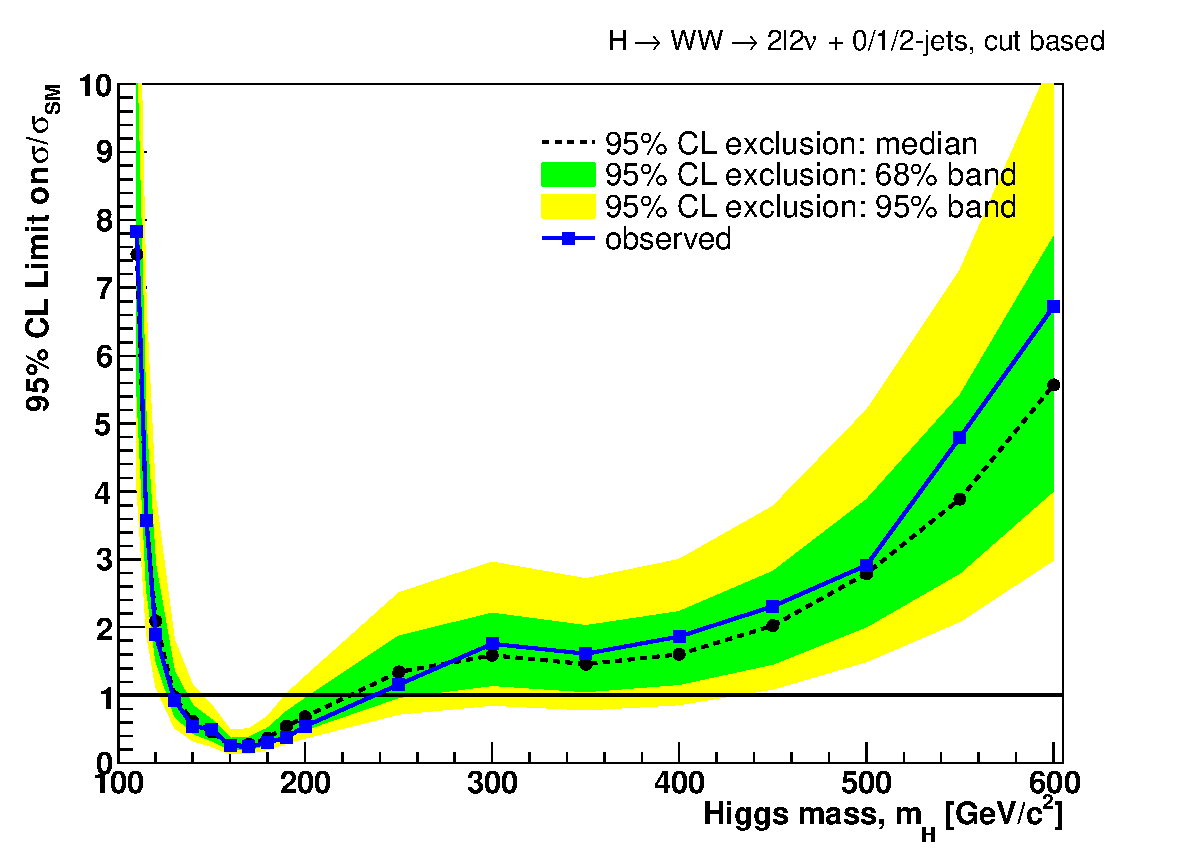
\includegraphics[width=.45\textwidth]{figures/limits_nj_cut-CLs-asymptotic_PostEPS.pdf}}
\subfigure[SM Higgs (shape-based)]{
\centering
\label{subfig:sm_cut_zoom}
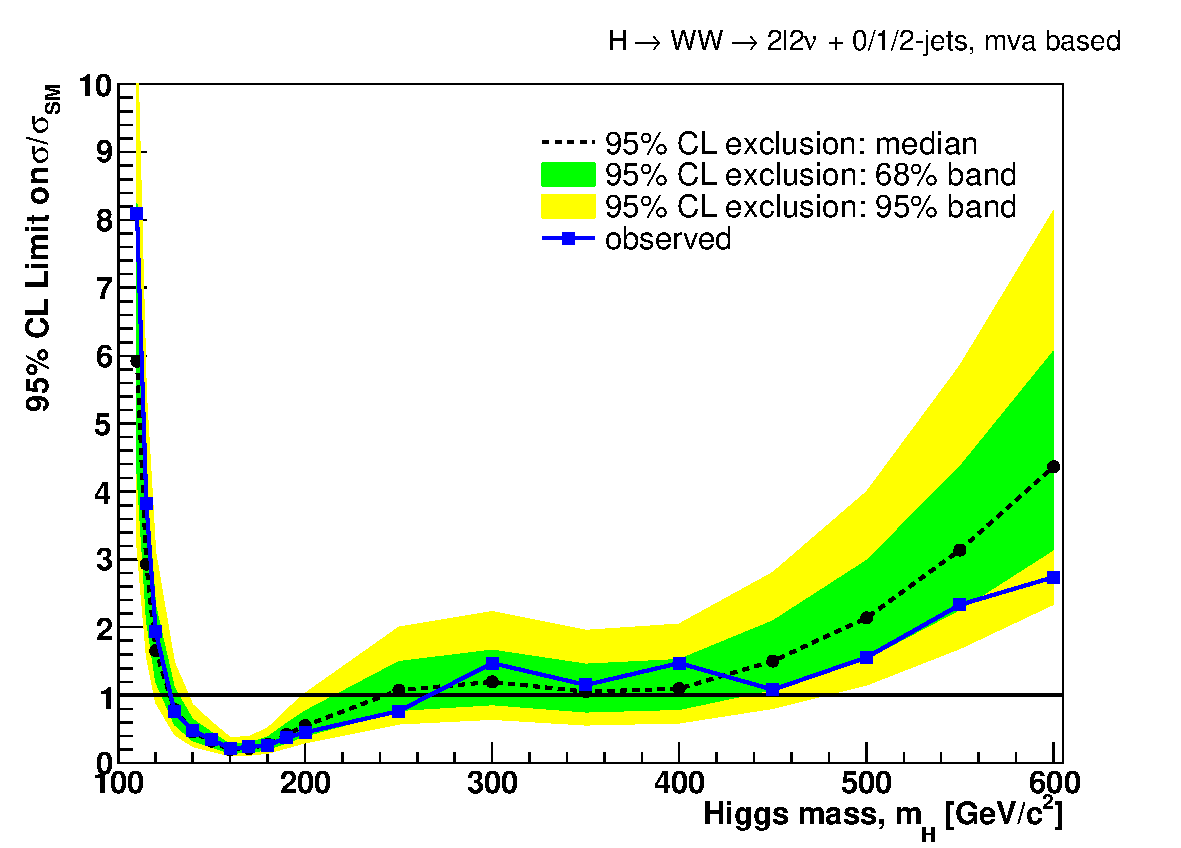
\includegraphics[width=.45\textwidth]{figures/limits_nj_shape-CLs-asymptotic_PostEPS.pdf}}

\caption{Expected and observed upper limits on the SM using Post-EPS dataset.}
\label{fig:uls_posteps}
\end{figure}

